\section{The irreducible length tail from signed cylinder estimates}
\label{R:alt:j}

This section derives the irreducible length tail using only the signed
cylinder estimates stated below and the elementary renewal identities.
The main difficulty is a lower bound: large mean length for finite chords
must force a long irreducible piece, even after the chords are converted
into bridges. We control the second length moment by closing chords into
polygons, and control the multiplicity of the conversion by folding arches
around a fixed irreducible piece.

\subsection{Finite inputs and the proof strategy}

We use ports on the triangular tiling of side one, with height measured in
whole tessellation layers and length equal to visited vertex count.
The finite inputs come from the signed cylinder representation
\cite[Section~2, Propositions~9.1--9.2 and Theorems~1.1--1.2]{RenewalSignedCompanion}.
We state them here in the form used below.
Let $\vartheta=\pi/8$.  If $K(a,b)$ is the positive critical chord kernel in
a convex tessellation polygon, its signed boundary balance is
\[
 \sum_b e^{3iT(a,b)/8}K(a,b)=1,
\]
where $T(a,b)$ is the total tangent turn of a chord from the inward edge
at $a$ to the outward edge at $b$.  Convexity gives
$|T(a,b)|\le\pi$, so the real coefficients are uniformly positive.
The same local identity cancels the two orientations of a self-collision
whose incoming stem lies outside its loop.  In the upper half-plane put
$H_\partial(d)=K(0,d)$ for the kernel to the port $d$ lattice units to the
right, and let $W_R$ be the mass of arches from one port reaching distance
at least $R$.  The finite boundary theorem gives
\begin{equation}\label{R:alt:j:finite-boundary}
 2\sin\vartheta\sum_{d\ge1}H_\partial(d)=1,
 \qquad W_R=R^{-1/4+o(1)}.
\end{equation}
For a finite convex tessellation polygon $D$ and a honeycomb vertex $v$
not adjacent to a boundary port, the raw critical visit mass summed over
all ordered first-exit boundary chords of $D$ through $v$, with both
sources and terminals summed, is comparable with absolute positive
constants to the sum of the three nesting partitions at its incident
face centers. Each nesting partition counts disjoint enclosing polygons
in $D$, with weight $2\rho^{|\lambda|}$ per polygon.
Writing $G_M(g)$ here for the companion's $G_{M/2}(g)$, where the full
physical period $M$ belongs to $4\mathbb N$ and the two marked faces are
half a period apart, we have
\begin{equation}\label{R:alt:j:finite-cylinder}
 G_M(2)=M^{1/6+o(1)}.
\end{equation}
The visit and localization theorems give the following bounds in a regular
hexagon $D_R$ of side $R$: the mass of ordered chords visiting the middle
disk of radius $R/10$ is at most $R^{3/4+o(1)}$, and their first length
mass is at least $R^{25/12-o(1)}$. Indeed, every chord visiting the middle
disk belongs to the companion's macroscopic chord ensemble, which gives
the mass upper bound. Its uniform raw visit mass at each middle vertex is
$R^{1/12+o(1)}$. Summing over the order $R^2$ vertices in the disk gives
the first-length lower bound. Finally the marked-polygon theorem gives
\begin{equation}\label{R:alt:j:polygon-input}
 \sum_{\substack{\lambda\ \text{modulo translations}\\
                   \operatorname{diam}\lambda\le Q}}
       \rho^{|\lambda|}|\lambda|^2\le Q^{2/3+o(1)}.
\end{equation}
Polygons in this display are simple, unoriented and unrooted, with each
lattice-translation class counted once. Counting both orientations changes
only a factor of two; rooting at every vertex would change the moment
being estimated. These finite inputs precede the renewal argument.
For an infinite concatenation, let $\gamma_0$ denote its starting port.

\begin{theorem}[Length tail from boundary folding]
\label{R:alt:j:theorem}
Under the irreducible critical bridge law $p$, the finite estimates above
imply
\[
 p(L\ge n)=n^{-9/16+o(1)}.
\]
They also give $p(H>r)=r^{-3/4+o(1)}$ and
$p(D>r)\le r^{-3/4+o(1)}$.  Consequently the iid infinite bridge satisfies
$|\gamma_n-\gamma_0|=n^{3/4+o(1)}$ and has
$R^{4/3+o(1)}$ vertices in a radius-$R$ disk, almost surely.
At every integer strip height $h$, the critical fixed-source,
free-terminal bridge law has length $h^{4/3+o(1)}$ in probability and
mean length $h^{4/3+o(1)}$.  Under the bridge law summed over heights with
weight $\rho^Le^{-L/t}$, length is $t^{1+o(1)}$ and diameter is
$t^{3/4+o(1)}$ in probability.
\end{theorem}

All masses in the proof have the positive weight $\rho^{\mathsf L}$ unless a tilt is explicitly
specified. Turning phases occur only in the identities used to compare
these masses.

The decisive comparison can be stated before the geometric details.
Sum over $H\le R\le2H$ and over ordered chords of $D_R$ visiting its middle
disk, and let $M_j(H)$ be the resulting mass with insertion
$\mathsf L^j$. The inputs give
\[
 M_0(H)\le H^{7/4+o(1)},\qquad M_1(H)\ge H^{37/12-o(1)}.
\]
We shall prove
\[
 M_2(H)\le H^{53/12+o(1)}.
\]
Removing chords shorter than $H^{4/3-\delta}$ does not remove the first
moment, and Cauchy--Schwarz then leaves long-chord mass
$H^{7/4-o(1)}$. Depending on their endpoint sides, these chords give
long bridge mass $H^{3/4-o(1)}$ summed over a height interval, or long arch
mass $H^{-1/4-o(1)}$ from a fixed source. Folding an arch at its highest
point makes a bridge. The additional estimate needed for this operation
bounds its weighted multiplicity by $H^{1/2+o(1)}$, uniformly after one
irreducible piece is prescribed. These powers will give the lower
irreducible tail $p(L\ge H^{4/3-\eta})\ge H^{-3/4-o(1)}$.

The proof develops the estimates in their dependency order. Boundary
balances first give strip masses, strip moments and a slit bound.
A two-source identity then controls pairs of ordered renewal arms;
this proves the uniform folding estimate. Finally we close the finite
chords, extract the lower tail, and apply the renewal identities to the
three laws in Theorem~\ref{R:alt:j:theorem}.

\subsection{Boundary comparisons and strip moments}

Levels are horizontal tessellation lines, with heights in units of their
spacing. Distances along a line are in side units. Let $b_h$ be the mass
of strict bridges from a fixed bottom port to the top of the infinite
height-$h$ strip, and put $b_0=1$. Let $a_j$ be the fixed-source
half-plane arch mass with maximum in layer $j$, the region between levels
$j-1$ and $j$. Its highest visited triangle is down-pointing and has
center at height $j-1/3$: an up-pointing triangle in that layer has only
one branch leading down and cannot be an internal maximum.
Write
\[
 A(d)=\sum_{q\ge d}H_\partial(q).
\]

\begin{lemma}[Comparison with a half-plane cap]\label{R:signed:cap}
In any convex tessellation domain, finite or infinite, the mass of chords
from a fixed port which reach distance at least $S$ from that port is at
most $C W_{cS}$, for absolute positive constants $c,C$. Convex boundary
balances extend to half-planes, strips and wedges by exhaustion.
\end{lemma}
\begin{proof}
First exhaust a tangent half-plane by aligned tessellation hexagons.
Boundary saturation in \eqref{R:alt:j:finite-boundary} and positive real
parts show that the artificial exits tend to zero. Artificial exits in
any smaller convex domain are a subset of these exits, so they too vanish.
This justifies its limiting boundary balance.

For the quantitative assertion, cut the domain by a tessellation hexagon
about a nearby lattice vertex, whose inner and outer radii about the source
lie between $cS$ and $S/2$. Subtract the balances before and after the cut.
A chord valid in both domains has the same terminal phase and cancels;
all remaining old chords are precisely those lost on imposing the cut.
Every chord reaching distance $S$ is among these lost chords. The new
exits lie on the cap, and convex positivity compares their mass with the
lost mass in both directions, with absolute constants. Their paths are
also cap exits in the cut tangent half-plane. Applying the same subtraction
there bounds their mass by the lost half-plane arch mass, at most
$W_{cS}$. The exhaustion argument above applies if the original domain
is infinite.
\end{proof}

\begin{lemma}[Boundary tails and bridge mass]\label{R:signed:strip-mass}
One has
\begin{equation}\label{R:alt:j:eq-br1}
 A(h)=h^{-1/4+o(1)},\qquad b_h=h^{-1/4+o(1)}.
\end{equation}
For a wedge of angle $60^\circ$ or $120^\circ$, a source on one ray at
apex distance at most $CH$ has mass at least $H^{-1/4-o(1)}$ to the other
ray. This lower bound is retained within distance $H^{1+\epsilon}$ of
the source, for every fixed $\epsilon>0$.
\end{lemma}
\begin{proof}
Consider first the $60^\circ$ wedge between the positive horizontal ray
and the ray at angle $\pi/3$, with source at half-integer coordinate
$a>0$ on the horizontal ray. Relative to the full upper half-plane,
let $L_<(a)$ and $L_>(a)$ be the lost masses to the left and right of the
source, including endpoints beyond the apex. Let $D(a,b)$ be the lost
mass when both endpoint coordinates are positive. Reversal gives
$D(a,b)=D(b,a)$.

The phases of a left base exit, a right base exit and an exit on the
other ray are respectively $e^{3i\vartheta}$, $e^{-3i\vartheta}$ and
$e^{i\vartheta}$. If $K_{\rm w}(a)$ is the mass to the other ray,
subtraction of the balances gives
\[
 e^{3i\vartheta}L_<(a)+e^{-3i\vartheta}L_>(a)
       =e^{i\vartheta}K_{\rm w}(a).
\]
Multiplication by $e^{-i\vartheta}$ and imaginary parts yield
$L_<(a)=\sqrt2 L_>(a)$. Summing this relation over $a\le R$ and using
symmetry of $D$ gives
\[
 (\sqrt2-1)\sum_{0<a<b\le R}D(a,b)
 +\sqrt2\sum_{0<a\le R<b}D(a,b)
   =\sum_{0<a\le R}A(\lceil a\rceil).
\]
The total loss is at most $CW_{ca}$ by Lemma~\ref{R:signed:cap}. For a
lower bound, take also the reflected wedge with its apex on the other
side of the source. Their intersection is a triangle of diameter $O(a)$.
An arch escaping this triangle is lost in at least one wedge; reflection
makes their loss masses equal. Thus the total loss in either wedge is
at least $cW_{Ca}$, and has exponent $-1/4$.

Since $L_>(a)=\sum_{b>a}D(a,b)$, the preceding identity is bounded above
and below by fixed multiples of $\sum_{a\le R}L_>(a)$. Consequently
\[
 \sum_{a\le R} A(\lceil a\rceil)=R^{3/4+o(1)}.
\]
Monotonicity gives the upper bound for $A(R)$. For the lower bound,
subtract the cumulative sum at $R$ from that at $R^{1+\delta}$ and bound
the difference above by $R^{1+\delta}A(R)$. Letting $\delta\downarrow0$
proves the first assertion in \eqref{R:alt:j:eq-br1}.

Half-plane--strip subtraction gives the exact relation
\[
 b_h=\sin\vartheta\sum_{j>h}a_j.
\]
An arch in this sum reaches distance comparable to $h$, so the cap bound
gives $b_h\le h^{-1/4+o(1)}$. To obtain the reverse bound, let
$K_{\rm w}(a,v)$ be the other-ray wedge kernel. Reversal and reflection
make it symmetric in $a,v$, and the balance above shows
$\sum_vK_{\rm w}(a,v)=a^{-1/4+o(1)}$. Cut the wedge at height $h$.
All exits with $v>Ch$ are lost, and the new exits have mass at most
$b_h$ per source. By symmetry,
\[
 \sum_{a\le R}\sum_{v>Ch}K_{\rm w}(a,v)
 \ge R^{3/4-o(1)}-h^{3/4+o(1)}.
\]
The subtracted term bounds the sum with $v\le Ch$ by summing first over
$v$ and then over all $a$. Therefore
\[
 Rb_h\ge c\bigl(R^{3/4-o(1)}-h^{3/4+o(1)}\bigr).
\]
Set $R=h^{1+\epsilon}$ and let $\epsilon\downarrow0$.

For either stated wedge angle, the missing same-side endpoints beyond
the apex have mass at least $A(CH)=H^{-1/4+o(1)}$. Its boundary balance
compares the total same-side loss with the other-ray mass, with fixed
positive constants. Lemma~\ref{R:signed:cap} removes at most
$H^{-(1+\epsilon)/4+o(1)}$ outside the prescribed radius, which is
negligible. This proves the confined assertion.
\end{proof}

\begin{lemma}[Strip moments and fixed-width summability]
\label{R:signed:strip-moments}
Let $H_h(d)$ be the strip same-side kernel at separation $d$. Then
\[
 m_B(h):=\sum_{\text{bridges of height }h}\mathsf L\rho^{\mathsf L}
       \le h^{13/12+o(1)},
\]
and the same upper bound holds for the first-length mass of strip arches.
Moreover,
\begin{equation}\label{R:alt:j:eq-br2}
 \sum_{d>0}d H_h(d)\le h^{3/4+o(1)}.
\end{equation}
At each fixed strip height, the total critical mass and first-length mass
of all walks from a fixed vertex staying in that strip are finite.
\end{lemma}
\begin{proof}
The interior visit identity bounds the sum of positive chord visits to
any non-boundary-adjacent vertex by a constant times its three incident
$+2$ nesting partitions. Each such one-face partition in the full strip
has square at most $G_M(2)$, for a physical period $M\asymp Ch$ divisible
by four in a transverse $60^\circ$ direction. To see the square, translate
one strip and its marked face to each of the two cylinder marks. For
large fixed $C$, the vertical separation of the half-period translates
exceeds the strip width. The two strips are disjoint, their cycles embed
without intersections, and every cycle separates the marks. Their
independent union is therefore counted by $G_M(2)$.

It follows from \eqref{R:alt:j:finite-cylinder} that the raw visit mass
at each such vertex is at most $h^{1/12+o(1)}$. This bound applies first
in finite convex strip exhaustions and then, by positivity, to genuine
strip chords. For a fixed source, sum visits along a horizontal row.
Horizontal translation identifies this sum with the sum over the
corresponding boundary sources at one representative vertex of that row;
it is bounded by the raw all-source visit estimate. There are $O(h)$
rows. Visits in a port-adjacent row can be charged, with bounded
multiplicity, to slant neighbors on the path that are not adjacent to
the boundary, when $h\ge2$. This proves the first-length bounds. Smaller
heights have finite masses and moments as well: append a fixed bridge
to reach a larger height; for arches use monotonicity.

For \eqref{R:alt:j:eq-br2}, cut the strip on a transverse $60^\circ$
tessellation line. Compare balances in the strip and in one remaining
side of this cut, then sum over bottom sources on that side. Retain only
same-side chords whose endpoints are on opposite sides of the cut;
all are lost. A chord with endpoint separation $d$ has exactly $d$ such
source placements, up to a fixed lattice factor. The total lost mass thus bounds the left
side of \eqref{R:alt:j:eq-br2}. It is controlled by new cut exits.
Reversing these paths gives, at each cut port of height $y$, a mass of
bottom exits at most $O(1)$, and at most $CW_{cy}$ when $y$ is bounded
away from zero, by Lemma~\ref{R:signed:cap}. Summing over $0\le y\le h$
gives $h^{3/4+o(1)}$.

We finally record why arbitrary fixed-width walks, needed in the slit
exhaustion below, are summable. Split such a walk at a global highest
vertex. On each resulting chain, cut at the last occurrence of its
lowest level, then the last highest level in the remainder, and continue.
Vertex heights in thirds of a layer are integral and change at every
step. The positive spans of these extremal pieces decrease strictly,
except possibly for equality of the first two. Thus the number of pieces
is bounded in terms of the strip height. Each piece can be extended at
its extreme ends to horizontal ports by adding at most one new vertex
per end, giving a bridge with bounded multiplicity and bounded weight
change. Drop avoidance between different pieces and compensate for shared
endpoints. There are finitely many possible lists of spans. For each list,
the mass and its first-length insertion are bounded by products of finite
bridge masses and moments. There are only finitely many possible rows of
the split vertex; after fixing a representative in that row, the original
initial vertex determines at most one horizontal translation. This proves
both asserted finiteness statements.
\end{proof}

\subsection{Slit estimates and ordered pairs of renewal arms}

The next estimates will control how many arches can fold into a bridge
containing a prescribed irreducible. We first bound paths that go around
the tip of a slit. We then use the same bound for pairs of bridge prefixes
whose endpoints are far apart at the shorter height.

\begin{lemma}[A slit bound uniform in the lower depth]\label{R:signed:slit}
In the strip between levels $-s_0$ and $L$, where $s_0,L$ are positive
integers, cut the bonds at ports on a horizontal ray from a tessellation
vertex to the right at level zero. The cut has upper and lower shores.
For an upper-shore source at distance $a=1/2,3/2,\ldots$ from the tip,
entering upward, let $V(a)$ be the mass of exits on the bottom wall. Then
\begin{equation}\label{R:alt:j:eq-br3}
 \sum_a V(a)\le L^{3/4+o(1)},
\end{equation}
uniformly in $s_0$.
\end{lemma}
\begin{proof}
The slit is attached to the exterior. A stem from its boundary still
approaches a first self-collision from outside the new loop, so the same
local cancellation proves the signed balance. Figure~\ref{R:alt:j:slit-figure} shows the domain. The following table gives
the boundary-determined turns from an upward-entering source; a thin
opening of the slit makes the concave tip turn $-\pi$ explicit. Put
$\theta_0=3\pi/8$.
\[
\begin{array}{c|ccccc}
\text{exit}&\text{upper left}&\text{upper right}&\text{top}
       &\text{bottom}&\text{lower shore}\\ \hline
T&\pi&-\pi&0&\pi&2\pi\\
e^{3iT/8}&e^{i\theta_0}&e^{-i\theta_0}&1
       &e^{i\theta_0}&e^{2i\theta_0}
\end{array}
\]
Compare with the isolated upper strip of height $L$. Let $E_<(a)$ and
$E_>(a)$ be the nonnegative gains to other upper-shore ports on the left
and right of the source, and let $E_T(a)$ be the gain to the top. Let
$A_0(a)$ be the reference mass to same-side endpoints left of the tip,
which are missing from the slit shore. Project the balance difference by
\[
 \mathcal P(w)=-\frac{\Im(e^{-2i\theta_0}w)}{\sin\theta_0}.
\]
It kills every lower-shore term, including a return to the same cut
location. The other coefficients give
\[
 E_<+V+2\cos\theta_0\,E_T
   =A_0+\frac{\sin(\pi/8)}{\sin\theta_0}E_>.
\]

These identities may first be written in remote finite truncations.
Lemma~\ref{R:signed:strip-moments} makes their exit errors vanish and
allows absolute summation over sources. For the latter assertion, every
gained or bottom-exiting path goes around the tip. Translate to a fixed
source and ignore the slit: its possible offsets relative to the tip
are at most a constant times its length. The fixed-width first-length
sum therefore bounds the summed gains and bottom exits.

Reversal of an upper-shore gained chord gives
$\sum_a E_<(a)=\sum_a E_>(a)$. Since
$\sin(\pi/8)/\sin\theta_0=\sqrt2-1<1$, summation and positivity imply
\[
 \sum_aV(a)\le\sum_aA_0(a)=\sum_{d>0}dH_L(d).
\]
Lemma~\ref{R:signed:strip-moments} proves the desired bound. Its right
side depends only on the upper height $L$, which explains the uniformity
in $s_0$.
\end{proof}

\begin{figure}[ht]
\centering
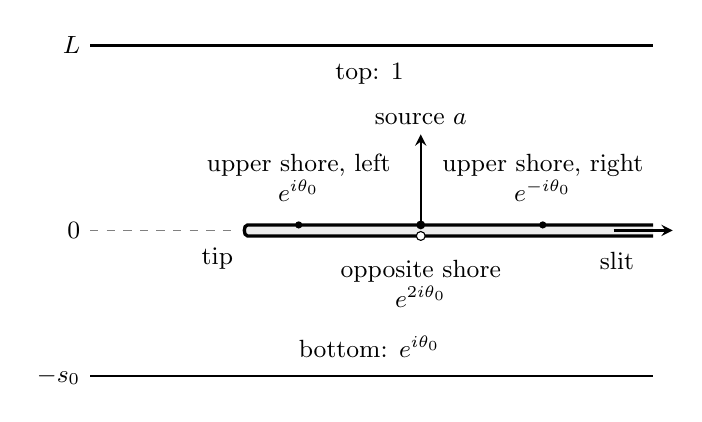
\begin{tikzpicture}[x=1cm,y=1cm,>=stealth,font=\small]
  \draw[thick] (-2,2.35)--(5.15,2.35);
  \draw[thick] (-2,-1.85)--(5.15,-1.85);
  \node[left] at (-2,2.35) {$L$};
  \node[left] at (-2,-1.85) {$-s_0$};
  \draw[dashed,gray] (-2,0)--(-.14,0);
  \node[left] at (-2,0) {$0$};
  \fill[gray!15] (0,.07)--(5.15,.07)--(5.15,-.07)--(0,-.07)
    to[out=180,in=180] (0,.07);
  \draw[very thick] (5.15,.07)--(0,.07)
    to[out=180,in=180] (0,-.07)--(5.15,-.07);
  \draw[->,thick] (4.65,0)--(5.4,0);
  \node[below left] at (-.06,-.1) {tip};
  \node[below right] at (4.35,-.15) {slit};
  \fill (2.2,.07) circle (1.6pt);
  \draw[fill=white] (2.2,-.07) circle (1.6pt);
  \draw[->,thick] (2.2,.12)--(2.2,1.22);
  \node[above] at (2.2,1.22) {source $a$};
  \fill (.65,.07) circle (1.3pt);
  \fill (3.75,.07) circle (1.3pt);
  \node[above,align=center] at (.65,.24)
    {upper shore, left\\$e^{i\theta_0}$};
  \node[above,align=center] at (3.75,.24)
    {upper shore, right\\$e^{-i\theta_0}$};
  \node[below,align=center] at (2.2,-.25)
    {opposite shore\\$e^{2i\theta_0}$};
  \node[below,align=center] at (1.55,2.24) {top: $1$};
  \node[above,align=center] at (1.55,-1.74)
    {bottom: $e^{i\theta_0}$};
\end{tikzpicture}
\caption{The slit domain and the exit phases for an upward-entering
source at distance $a$ from the tip, where $\theta_0=3\pi/8$.
The shores are separated in the drawing to distinguish the two ports
at each cut bond.  A chord to the opposite shore has total tangent turn
$2\pi$; its phase is therefore removed by projection perpendicular to
$e^{2i\theta_0}$.}
\label{R:alt:j:slit-figure}
\end{figure}

\begin{lemma}[Two sources and positive boundary kernels]
\label{R:signed:two-source}
Let $K$ be the positive chord kernel in a convex tessellation polygon.
For adjacent ports $a,b$ in counterclockwise order on a straight boundary
segment and another port $e$, with cyclic order $a<b<e$, let
$K_2(ac,bd)$ denote the mass of mutually vertex-disjoint chord pairs.
Put $r=e^{2i\vartheta}$ and $s=3/8$. Then
\begin{equation}\label{R:alt:j:eq-br4}
K(a,e)-rK(b,e)
 =\sum_{b<d<e}e^{isT(b,d)}K_2(ae,bd)
 -r\sum_{e<c<a}e^{isT(a,c)}K_2(ac,be).
\end{equation}
Consequently same-side kernels decrease as the terminal port moves away
from a fixed source. For every fixed small $\epsilon>0$, the half-plane
kernel confined within distance $H^{1+5\epsilon}$ of its source satisfies
\begin{equation}\label{R:alt:j:eq-br5}
K_{\rm conf}(c,b)\ge H^{-5/4-C\epsilon-o(1)}
\qquad(1\le |b-c|\le H^{1+3\epsilon}).
\end{equation}
\end{lemma}
\begin{proof}
Because $a,b$ lie on the same straight side, $T(a,e)=T(b,e)$; give both
trunks the common phase $e^{isT(a,e)}$ during the following exploration.
Fix a trunk from $a$ to $e$ and grow a turning-weighted stem from $b$,
stopping at its first trunk contact as well as at boundary exits. Compare
this with trunk $b$ to $e$ and stem from $a$. Self-collisions cancel by
the local rule. A contact term is an embedded Y tree with outward arms
in cyclic order $a,b,e$. At its junction, the turn from the $a$ arm onto
the $e$ arm is $+\pi/3$, whereas from the $b$ arm it is $-\pi/3$.
The other turns and all vertex weights agree, so the ratio of the two
contact phases is $e^{is(2\pi/3)}=r$. This also covers immediate contact.
After multiplying the second exploration by $r$, all contact terms cancel.
The remaining disjoint boundary exits have exactly the two cyclic ranges
in \eqref{R:alt:j:eq-br4}; division by the common trunk phase gives that
identity. In strip exhaustions, remote disjoint exits vanish by product
domination and the cap bound.

If $e$ lies beyond $b$ on the same base segment, multiply the identity
by $e^{3i\vartheta}$ and take imaginary parts. The first sum has zero
imaginary part. In the subtracted sum the sine phases are nonnegative,
since $5\vartheta+sT\in[2\vartheta,8\vartheta]$. As
$\sin3\vartheta=\sin5\vartheta>0$, this gives $K(a,e)\le K(b,e)$.
Reversal makes it outward decrease of the terminal from a fixed source;
a tessellation reflection gives the other direction.

To prove the confined lower bound, use a tangent half-hexagonal cap
whose radius is a small constant times $H^{1+5\epsilon}$. Along its base,
the sum of kernels to ports beyond distance $H^{1+4\epsilon}$ is at least
the half-plane tail $A(H^{1+4\epsilon})$ minus the lost mass
$CW_{cH^{1+5\epsilon}}$. By Lemmas~\ref{R:signed:cap}
and~\ref{R:signed:strip-mass}, the second term is negligible and the first
has exponent $-(1+4\epsilon)/4$. There are $O(H^{1+5\epsilon})$ ports
on the cap base. The outward monotonicity just proved bounds the kernel
to every nearer port below by this sum divided by that number. The cap
lies inside the required confinement radius, giving
\eqref{R:alt:j:eq-br5}.
\end{proof}

\begin{lemma}[Top endpoints of two bridges]\label{R:signed:bridge-pair}
Take adjacent bottom ports $a,b$, ordered left to right. Let $b_h(e)$ be
the height-$h$ top kernel from $a$, and put
$D_h(c,d)=K_2(ac,bd)$ for top ports $c<d$, in left-to-right order. Then
\[
 b_h(e)-b_h(e-1)=\sum_{d>e}D_h(e,d)-\sum_{c<e}D_h(c,e),
 \qquad b_h(e)=\sum_{c\le e<d}D_h(c,d),
\]
and
\begin{equation}\label{R:alt:j:eq-br6}
 \sum_{h\ge H}\sum_{c<d}D_h(c,d)\le H^{-1/4+o(1)}.
\end{equation}
\end{lemma}
\begin{proof}
Apply the imaginary-part projection in the preceding proof with $e$ on
the top wall. Bottom exits to the right of $b$ and to the left of $a$
vanish. The top coefficients agree because
$\sin3\vartheta=\sin5\vartheta$, giving the difference identity.
Summing it from the left end of the strip gives the second identity;
the kernel tends to zero at infinity by summability.

For the last bound, join the adjacent bottom ports below the strip by a
three-center arch. Together with the two bridges this gives a downward
half-plane arch from $c$ to $d$. Translate its first port to a fixed
source. The connector has a unique deepest vertex, so the output recovers
the connector, the translation and the original height. Thus the map is
injective over all $h$, with constant weight factor $\rho^3$. Its image
reaches distance at least a constant times $H$, and
\eqref{R:alt:j:finite-boundary} proves the bound.
\end{proof}

We now pass to irreducible pieces, still without any lower length-tail
estimate. Unique decomposition at once-crossed levels gives
\[
 B(z)=\sum_{h\ge0}b_hz^h=\frac1{1-I(z)},\qquad
 I(z)=\sum_{\gamma\in\mathcal I}\rho^{L(\gamma)}z^{H(\gamma)}.
\]
Lemma~\ref{R:signed:strip-mass} gives
$B(e^{-1/H})=H^{3/4+o(1)}$; letting $z\uparrow1$ proves $I(1)=1$.
Thus the critical irreducible weights define the same law $p$ as in
Proposition~\ref{R:renew:factorization}. Write
$\mathsf H,\mathsf X,\mathsf L$ for a block's height, signed horizontal
displacement and length, and let $S$ be its horizontal coordinate range.
Its diameter is at most $C(\mathsf H+S)$.

It will be convenient to name the normalized law of all finite bridges
with weight $\rho^{\mathsf L}z^{\mathsf H}$, including the empty bridge:
call it $\mathbb Q_z$. Under $\mathbb Q_z$, the number of pieces is
geometric with probabilities $(1-I(z))I(z)^k$, $k\ge0$, and, given this
number, their shapes are independent with law
\[
 p_z(d\gamma)=I(z)^{-1}z^{H(\gamma)}p(d\gamma).
\]
This statement concerns different pieces; no independence of the
coordinates within one piece is asserted.

\begin{lemma}[Increment estimates before the lower length bound]
\label{R:signed:increments}
Under $p$,
\begin{equation}\label{R:alt:j:eq-br7}
 \mathbb P_p(\mathsf H>t)=t^{-3/4+o(1)},\qquad
 \mathbb P_p(S>t)\le t^{-3/4+o(1)},\qquad
 \mathbb P_p(\mathsf L>n)\le n^{-9/16+o(1)}.
\end{equation}
In addition, $\mathbb P_p(|\mathsf X|>t)=t^{-3/4+o(1)}$.
\end{lemma}
\begin{proof}
The height deficit is
$\mathbb E_p(1-e^{-\mathsf H/t})=t^{-3/4+o(1)}$, giving the height upper
tail and $\mathbb E[\mathsf H;\mathsf H\le t]\le t^{1/4+o(1)}$.
Evaluate the deficit at $t^{1+\epsilon}$. Heights at most $t$ contribute
only $t^{-3/4-\epsilon+o(1)}$, which is smaller than the deficit
$t^{-3(1+\epsilon)/4+o(1)}$. This proves the lower tail as
$\epsilon\downarrow0$.

Call a block wide if $S>t$, and put
$u=\mathbb E_p[z^{\mathsf H};S>t]$. A bridge containing such a block is
itself wide, so at each height its mass is at most $CW_{ct}$ by the cap
bound. Under $\mathbb Q_z$, the probability of at least one wide block
is exactly
\[
 \frac{B(z)u}{1+B(z)u}.
\]
Take $z=e^{-1/H}$ with $H=t^{1-\epsilon}$. This probability is at most
$CHW_{ct}/B(z)=o(1)$, and hence
$u\le H^{-1/2+o(1)}t^{-1/4+o(1)}$. On $\mathsf H\le H$ the tilt is
bounded below. Add the height-tail bound on the complement and let
$\epsilon\downarrow0$ to obtain the span bound.

The marked-reward identity gives
\[
 \sum_hm_B(h)z^h=B(z)^2\mathbb E_p[\mathsf Lz^{\mathsf H}],
 \qquad \mathbb E_p[\mathsf L e^{-\mathsf H/H}]
       \le H^{7/12+o(1)}.
\]
Splitting according to $\mathsf H>n^{3/4}$ and applying Markov to the
remaining length gives the upper length tail in
\eqref{R:alt:j:eq-br7}.

It remains to prove that the signed displacement has a matching lower
tail. By Lemma~\ref{R:signed:bridge-pair}, bridge weights to any endpoint
windows of size $G$ per row, summed over $R\le h\le2R$, are at most
$C(G+1)R^{-1/4+o(1)}$. For $z=e^{-1/R}$, the whole height bin has
$\mathbb Q_z$-probability $R^{-o(1)}$, whereas the part with
$|\mathsf X_{\rm total}|\le R^{1-\epsilon}$ has probability at most
$R^{-\epsilon+o(1)}$. Thus displacement larger than this threshold has
at least subpower probability.

If every piece had displacement at most $t_*=R^{1-\delta}$, with
$\epsilon\ll\delta$, such a total displacement would be superpolynomially
unlikely. Here are the estimates. Reflection preserves height and
reverses displacement, so the truncated increments
$\mathsf X_{\rm trunc}=\mathsf X\mathbf1_{\{|\mathsf X|\le t_*\}}$
are centered under $p_z$. Their variance is at most $t_*^{5/4+o(1)}$ by the
span tail. The geometric number of pieces exceeds
$R^{3/4+c\delta}$ with superpolynomially small probability for small fixed
$c>0$. For $|v|\le1/t_*$,
\[
 \log\mathbb E_{p_z}e^{v\mathsf X_{\rm trunc}}
   \le C v^2\mathbb E_{p_z}\mathsf X_{\rm trunc}^2.
\]
Both the displacement threshold divided by $t_*$ and its square divided
by the resulting total variance grow as positive powers of $R$.
Exponential Markov therefore gives the claimed negligible probability.
A union bound, using the geometric mean $R^{3/4+o(1)}$, now forces
\[
 \mathbb E_p[z^{\mathsf H};|\mathsf X|>R^{1-\delta}]
       \ge R^{-3/4-o(1)}.
\]
Let $\delta\downarrow0$ and combine with the span upper tail.
\end{proof}

\begin{lemma}[Two ordered renewal arms]\label{R:signed:two-arms}
Start independent infinite $p$-sequences at adjacent bottom ports,
designated left and right. Let $P_m$ be the following event:
\begin{itemize}
\item the paths formed by the first $m$ pieces of the two arms are disjoint;
\item for each pair of positive renewal indices at most $m$, if their
heights are $n\le p$, every crossing of line $n$ by the height-$p$ prefix
lies strictly on its designated side of the other arm's endpoint at $n$.
When $n=p$, this means that the two endpoints are ordered.
\end{itemize}
Then
\begin{equation}\label{R:alt:j:eq-br8}
 p_m:=\mathbb P(P_m)\le m^{-1+o(1)}.
\end{equation}
\end{lemma}
\begin{proof}
Fix a small $\delta>0$, and set
\[
 L=\lceil m^{4/3+\delta}\rceil,\qquad G=m^{4/3-\delta}.
\]
We first show that, outside a superpolynomially small event, on each arm
at most $m/4$ renewal endpoints lie within horizontal distance $G$ of the
pertinent extreme crossing of the other full infinite path at that height.
The pertinent crossing is the leftmost on the right arm or the rightmost
on the left arm; it exists because the path reaches every height.

Condition on the other path. Divide the renewal indices into residue
classes modulo $m_0=\lfloor m^{1-c\delta}\rfloor$, with a small fixed
$c>0$. Successive sampled endpoints in one class are separated by a
fresh chunk of $m_0$ independent pieces. By the displacement lower tail
in Lemma~\ref{R:signed:increments}, such a chunk contains a positive
power of $m$ increments with magnitude greater than $2G$, except with
probability tending to zero. Conditional on all chunk heights and
absolute displacements, their nonzero signs are independent fair signs.
The target crossing position depends on the heights and the other path,
but not these signs.

If there are $k$ increments of magnitude greater than $2G$, their signed
sum lands in an interval of width $2G$ with probability at most
$C/\sqrt{k}$. Indeed, after fixing the other signs, the subsets of positive
large signs that yield a sum in that interval form an antichain: adding
one such sign changes the sum by more than $4G$. Counting maximal chains
bounds its size by the middle binomial coefficient. Thus the conditional
window probability at each sampled endpoint tends uniformly to zero.
Successive conditioning makes a positive fraction of hits in any residue
class exponentially unlikely in $m/m_0$. Union over the classes proves
the assertion about at most $m/4$ close endpoints; the initial incomplete
chunk costs at most $m_0=o(m)$ indices.

Suppose now that $P_m$ holds, both total heights are at most $L$, and the
exception above does not occur. There are at least $cm^2$ pairs of renewal
indices for which the two prefixes are disjoint and their gap at the
shorter height exceeds $G$. Crossings there by the longer prefix equal
those by its full path: later pieces lie strictly above its endpoint.
We claim that the expected number of all such height-bounded pairs is
\begin{equation}\label{R:signed:gap-pairs}
 O(1)+O(L^{7/4+o(1)}/G).
\end{equation}
Summing over renewal prefixes gives ordinary bridge weights. Equal-height
pairs have bounded total mass by \eqref{R:alt:j:eq-br6}. For unequal
heights, fix their difference $s_0=p-n>0$ and which arm is shorter.
Join their adjacent bottom starts by the three-center connector used in
Lemma~\ref{R:signed:bridge-pair}.

At row $n$, choose a tessellation vertex between the shorter endpoint and
the extreme crossing of the longer prefix. The gap gives at least $cG$
choices. From that tip cut the horizontal ray pointing away from the
longer path's crossings, through the shorter endpoint. The joined path
avoids the slit: the shorter bridge is strict below its endpoint, and
all crossings of the longer bridge at this row are on the other side.
It starts at the slit shore, goes toward the connector, and terminates
on the line of height $p$.

The map is illustrated in Figure~\ref{R:alt:j:pair-slit-figure}.
Send the tip $(t,n)$ to the origin. If the shorter endpoint is on the
right, use $(x',y')=(x-t,n-y)$; if it is on the left, use
$(x',y')=(t-x,n-y)$. These tessellation symmetries make the slit rightward
and the initial shore upper. The endpoint is on $y'=-s_0$, while the
unique highest vertex, on the connector, has $y'=n+2/3$. The path is
therefore counted by the slit estimate with upper wall $L+1$. Conversely,
its unique highest vertex recovers $n$, the connector and the original
translation, and hence both bridges and the chosen tip. For the fixed
assignment this map is injective, with a fixed weight factor. Summing
\eqref{R:alt:j:eq-br3} over the slit sources and dividing by the $cG$
tip choices bounds the pair mass, already summed over $n\le L$, by
$CL^{3/4+o(1)}/G$. Sum over the at most $L$ height differences to obtain
\eqref{R:signed:gap-pairs}.

Division by $cm^2$ now bounds $p_m$ in the restricted height range by
$m^{-1+C\delta+o(1)}$. To remove that restriction, set
$t=m^{4/3+\delta/2}$. Exponential Markov at $1/t$, together with
$\mathbb E[\mathsf H;\mathsf H\le t]\le t^{1/4+o(1)}$, shows that a
sum of $m$ heights exceeding $L$ with no increment above $t$ has
superpolynomially small probability. A height above $t$ at index $j$
on either arm is independent of $P_{j-1}$. Thus
\[
 p_m\le Cm^{-1+C'\delta+o(1)}
       +Cm^{-1-c'\delta}\sum_{j<m}p_j,
 \qquad p_0=1,
\]
for some $c'>0$. Induction gives $p_m=O_\eta(m^{-1+\eta})$ whenever
$\eta>C'\delta$: under this bound the second term is
$O(m^{-1+\eta-c'\delta})$. Choose $\delta$ arbitrarily small to obtain
\eqref{R:alt:j:eq-br8}.
\end{proof}

\begin{figure}[ht]
\centering
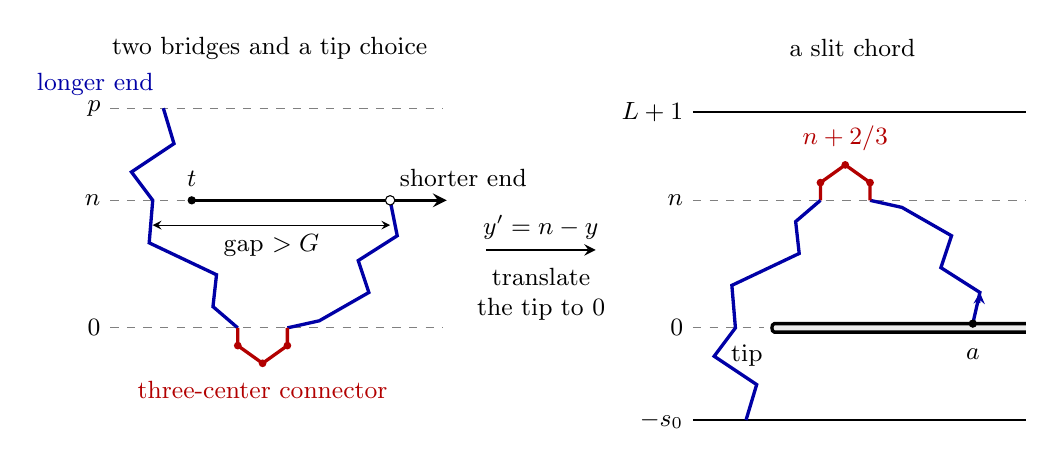
\begin{tikzpicture}[x=.9cm,y=.9cm,>=stealth,font=\small]
  \begin{scope}
    \node[align=center] at (1.1,3.95) {two bridges and a tip choice};
    \foreach \y/\lab in {0/{0},1.8/{n},3.1/{p}}
      {\draw[dashed,gray] (-1.15,\y)--(3.55,\y);
       \node[left] at (-1.15,\y) {$\lab$};}
    \draw[very thick,blue!65!black] (.65,0)--(.3,.3)--(.35,.75)
      --(-.6,1.2)--(-.55,1.8)--(-.85,2.2)--(-.25,2.6)--(-.4,3.1);
    \draw[very thick,blue!65!black] (1.35,0)--(1.8,.1)--(2.5,.5)
      --(2.35,.95)--(2.9,1.3)--(2.8,1.8);
    \draw[very thick,red!70!black] (.65,0)--(.65,-.25)
      --(1,-.5)--(1.35,-.25)--(1.35,0);
    \foreach \x/\y in {.65/-.25,1/-.5,1.35/-.25}
      {\fill[red!70!black] (\x,\y) circle (1.4pt);}
    \draw[very thick,->] (0,1.8)--(3.6,1.8);
    \fill (0,1.8) circle (1.5pt);
    \draw[fill=white] (2.8,1.8) circle (1.7pt);
    \node[above] at (0,1.86) {$t$};
    \node[above right] at (2.8,1.86) {shorter end};
    \node[below,red!70!black] at (1,-.62) {three-center connector};
    \draw[<->] (-.55,1.45)--(2.8,1.45)
      node[midway,below] {gap $>G$};
    \node[above left,blue!65!black] at (-.4,3.15) {longer end};
  \end{scope}
  \draw[->,thick] (4.15,1.1)--(5.7,1.1)
    node[midway,above,align=center] {$y'=n-y$};
  \node[below,align=center] at (4.93,.98) {translate\\the tip to $0$};
  \begin{scope}[xshift=7.4cm]
    \node[align=center] at (1.1,3.95) {a slit chord};
    \draw[thick] (-1.15,3.05)--(3.55,3.05);
    \draw[thick] (-1.15,-1.3)--(3.55,-1.3);
    \node[left] at (-1.15,3.05) {$L+1$};
    \node[left] at (-1.15,-1.3) {$-s_0$};
    \draw[dashed,gray] (-1.15,1.8)--(3.55,1.8);
    \node[left] at (-1.15,1.8) {$n$};
    \draw[dashed,gray] (-1.15,0)--(-.14,0);
    \node[left] at (-1.15,0) {$0$};
    \fill[gray!15] (0,.06)--(3.55,.06)--(3.55,-.06)--(0,-.06)
      to[out=180,in=180] (0,.06);
    \draw[very thick] (3.55,.06)--(0,.06)
      to[out=180,in=180] (0,-.06)--(3.55,-.06);
    \draw[very thick,blue!65!black] (2.8,.06)--(2.9,.5)--(2.35,.85)
      --(2.5,1.3)--(1.8,1.7)--(1.35,1.8);
    \draw[very thick,red!70!black] (1.35,1.8)--(1.35,2.05)
      --(1,2.3)--(.65,2.05)--(.65,1.8);
    \foreach \x/\y in {.65/2.05,1/2.3,1.35/2.05}
      {\fill[red!70!black] (\x,\y) circle (1.4pt);}
    \draw[very thick,blue!65!black] (.65,1.8)--(.3,1.5)--(.35,1.05)
      --(-.6,.6)--(-.55,0)--(-.85,-.4)--(-.25,-.8)--(-.4,-1.3);
    \fill (2.8,.06) circle (1.5pt);
    \draw[->,blue!65!black,thick] (2.89,.35)--(2.9,.5);
    \node[below] at (2.8,-.16) {$a$};
    \node[above,red!70!black] at (1,2.36) {$n+2/3$};
    \node[below left] at (-.03,-.1) {tip};
  \end{scope}
\end{tikzpicture}
\caption{The pair-to-slit map when the shorter arm is on the right.
Choose a tessellation vertex $t$ in the gap at height $n$, and direct
the slit through the shorter endpoint.  After reflection across that
level and translation of the tip, the shorter endpoint is an upper-shore
source and the longer endpoint is on the bottom line
$-s_0=-(p-n)$.  The unique maximum, at height $n+2/3$, identifies the
connector and recovers $n$.  If the shorter arm is on the left, a
half-turn about $t$ gives the same orientation.  Heights and paths are
schematic, and the two slit shores are separated only for display.}
\label{R:alt:j:pair-slit-figure}
\end{figure}

\subsection{Folding uniformly around a prescribed irreducible}

Fold a half-plane arch of exact maximum layer $k$ at its leftmost highest
down triangle. Split there, ending the first arm and starting the second
at the port above that triangle on line $k$, and reflect the second arm
across that line. The result is a height-$2k$ bridge, with a renewal at
$k$. The highest triangle was counted twice, so the folded weight is
$\rho$ times the arch weight. Unfolding at that middle renewal recovers
the arch, making this map injective.

Call a segment of an ordinary bridge \emph{valid} if its endpoints and
middle are renewal positions, at heights $c-k,c,c+k$, and it is the image
of this fold up to translation. Endpoints of the whole bridge are allowed.
Fix positive constants $c_1,C_1,C_2$ and a small $\epsilon>0$. Let $K$ count
valid segments whose half-height satisfies
\[
 c_1H\le k\le H^{1+C_1\epsilon}.
\]
The essential bound is uniform in the shape and length of a single fixed
irreducible; this is what will permit marking a long block later.

\begin{lemma}[Folding with a fixed irreducible]\label{R:signed:folding}
Fix an irreducible $\xi$ of height $d$. Place independent
$\mathbb Q_z$ bridges below and above it, translating $\xi$ to the joining
port, where $z=e^{-1/T}$ and $T=H^{1+C_2\epsilon}$. Write $\mathbb E^*_\xi$
for this law. Uniformly in $\xi$,
\begin{equation}\label{R:alt:j:eq-br9}
 \mathbb E^*_\xi K\le H^{1/2+O(\epsilon)+o(1)}.
\end{equation}
\end{lemma}
\begin{proof}
First count valid segments wholly outside $\xi$. Marking such a segment
in either exterior bridge gives two ordinary bridge factors and the folded
arch factor. One bridge normalization cancels, so this contribution is at
most
\[
 2\rho B(z)\sum_{k\text{ in range}}a_kz^{2k}
 \le 2\rho B(z)\sum_{k\ge c_1H}a_k
 \le H^{1/2+O(\epsilon)+o(1)}.
\]
The last inequality uses $B(z)=T^{3/4+o(1)}$ and the arch radius tail.

Every other valid segment contains the whole defect. Its middle renewal
cannot lie strictly inside an irreducible. Suppose first that this renewal
is $l\ge0$ levels below the start of $\xi$; the other case follows by
reversal and height reflection, which preserve the leftmost rule and
replace $\xi$ by a fixed transformed defect if necessary.

Here is the normalization cancellation for these segments. Cut at their
two endpoint renewals. The ordinary pieces outside the segment are free
and contribute $B(z)^2$, canceling the two exterior normalizations. Thus
for this orientation their contribution to $\mathbb E^*_\xi K$ is the sum,
over valid internal segments containing the fixed defect, of
\[
 \rho^{L(\text{segment})-L(\xi)}z^{2k-d}.
\]
There is no weight for the prescribed defect in this expression and no
sum over an independently chosen joining port. Unfolding the segment
at its middle gives two arms of height $k$: one ordinary bridge, and
one ordinary bridge of height $l$, followed by $\xi$, followed by an
ordinary bridge of height $k-l-d$. The pieces have total ordinary height
$2k-d$, as in the displayed weight. Reversed or reflected ordinary pieces
can be rooted at their first port by translation. Figure~\ref{R:alt:j:fold-figure}
shows these heights.

\begin{figure}[ht]
\centering
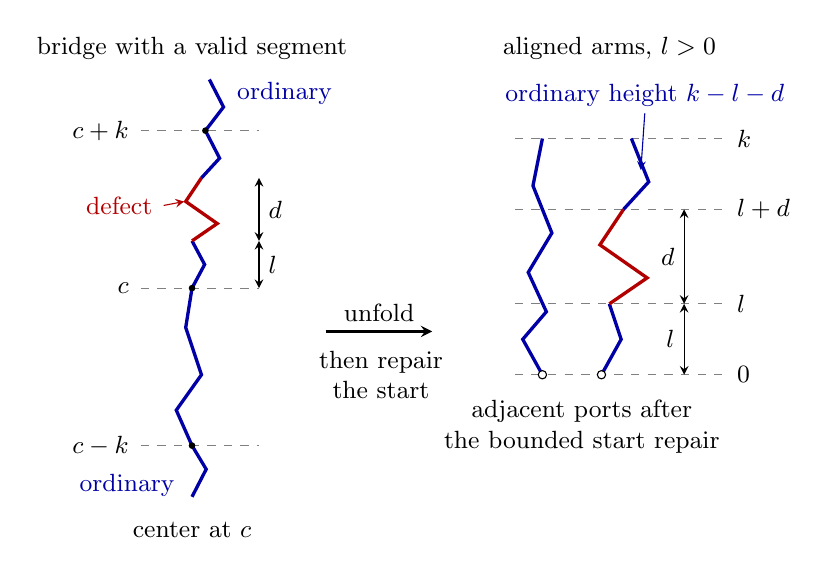
\begin{tikzpicture}[x=1cm,y=1cm,>=stealth,font=\small]
\begin{scope}[xshift=1.4cm]
\node[align=center]at(0,3.05){bridge with a valid segment};
\foreach \y/\lab in {-2/{c-k},0/{c},2/{c+k}}
 {\draw[dashed,gray](-.65,\y)--(.85,\y);
  \node[left]at(-.68,\y){$\lab$};}
\draw[very thick,blue!65!black] (0,-2.65)--(.18,-2.3)--(0,-2)
 --(-.2,-1.55)--(.12,-1.1)--(-.08,-.5)--(0,0)
 --(.16,.3)--(0,.6);
\draw[very thick,red!70!black] (0,.6)--(.32,.82)--(-.08,1.1)--(.12,1.4);
\draw[very thick,blue!65!black] (.12,1.4)--(.35,1.65)--(.17,2)
 --(.4,2.3)--(.22,2.65);
\foreach \x/\y in {0/-2,0/0,.17/2}{\fill(\x,\y)circle(1.2pt);}
\node[left,blue!65!black]at(-.1,-2.5){ordinary};
\node[right,blue!65!black]at(.45,2.48){ordinary};
\node[left,red!70!black]at(-.38,1.05){defect};
\draw[red!70!black,thin,->](-.36,1.05)--(-.10,1.10);
\draw[<->](.85,0)--(.85,.6)node[midway,right]{$l$};
\draw[<->](.85,.6)--(.85,1.4)node[midway,right]{$d$};
\node[below,align=center]at(0,-2.85){center at $c$};
\end{scope}
\draw[->,thick](3.1,-.55)--(4.45,-.55)
 node[midway,above,align=center]{unfold};
\node[align=center]at(3.8,-1.1){then repair\\the start};
\begin{scope}[xshift=5.5cm,yshift=-1.1cm]
\node[align=center]at(1.2,4.15){aligned arms, $l>0$};
\foreach \y/\lab in {0/{0},.9/{l},2.1/{l+d},3/{k}}
 {\draw[dashed,gray](.0,\y)--(2.65,\y);
  \node[right]at(2.7,\y){$\lab$};}
\draw[very thick,blue!65!black] (.35,0)--(.1,.45)--(.4,.8)
 --(.17,1.3)--(.47,1.8)--(.23,2.4)--(.35,3);
\draw[very thick,blue!65!black] (1.1,0)--(1.35,.45)--(1.2,.9);
\draw[very thick,red!70!black] (1.2,.9)--(1.68,1.23)--(1.08,1.65)--(1.38,2.1);
\draw[very thick,blue!65!black] (1.38,2.1)--(1.7,2.45)--(1.48,3);
\foreach \x in {.35,1.1}{\draw[fill=white](\x,0)circle(1.5pt);}
\draw[<->](2.15,0)--(2.15,.9)node[midway,left]{$l$};
\draw[<->](2.15,.9)--(2.15,2.1)node[midway,left]{$d$};
\node[align=left,blue!65!black]at(1.65,3.55){ordinary height $k-l-d$};
\draw[blue!65!black,thin,->](1.65,3.32)--(1.6,2.6);
\node[below,align=center]at(.85,-.2){adjacent ports after\\the bounded start repair};
\end{scope}
\end{tikzpicture}
\caption{Unfolding a valid segment containing a fixed irreducible defect, in the case $l>0$ and $l+d\le k$. The ordinary pieces outside the segment are omitted on the right. The red defect is unchanged; the bounded repair acts at the common start and produces the adjacent disjoint starts shown on the right. Heights are schematic and individual lattice edges are suppressed. The two exterior factors $B(z)$ cancel the normalizations by the cutting argument in the text, independently of this drawing.}
\label{R:alt:j:fold-figure}
\end{figure}

If $l=0$, dropping avoidance already bounds the aligned arm sum by
$T^{1/2+o(1)}$, using the squared-sum estimate below. Suppose $l>0$.
The unfolded arms initially meet only at their common port and first
down triangle, and take its distinct slant branches. They must be turned
into disjoint arms from adjacent ports before Lemma~\ref{R:signed:two-arms}
can be used.

Orient the unfolding downward and put its common port at $P=(0,0)$.
Write $h_0=\sqrt3/2$. The first down center is $D=(0,-h_0/3)$;
the left branch next visits $U=(-1/2,-2h_0/3)$. Replace the initial
portion $P,D,U$ of this branch by
\[
 P_-=(-1,0),\qquad D_-=(-1,-h_0/3),\qquad U.
\]
These are actual neighboring ports and centers, as shown in
Figure~\ref{R:alt:j:start-repair}. The center $D_-$ is unused by both
arms, because $D$ was chosen as the leftmost visited highest down
triangle of the arch. From $U$ the next edge cannot return to $D$ or
visit $D_-$, so it continues downward. The replacement therefore preserves
self-avoidance and makes the two arms disjoint. It substitutes one vertex
for one vertex, preserving each length and weight. All changed edges lie
at depths less than one; every positive integral-depth crossing and its
order is unchanged. Since $l\ge1$, the fixed defect is untouched.

The inverse restores the left initial portion using the unchanged right
port and first center. Keep the finitely many choices of arm and symmetry
as separate assignments. After reanchoring the adjacent starts at fixed
ports, the unchanged far endpoint and the original anchor determine the
translation back. This gives bounded inverse multiplicity with no
height-dependent factor.

\begin{figure}[ht]
\centering
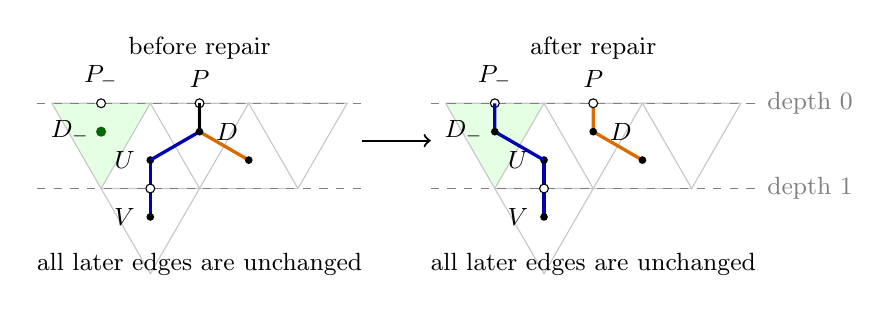
\begin{tikzpicture}[x=1.25cm,y=1.25cm,font=\small,
  lattice/.style={gray!45,thin},
  leftarm/.style={blue!70!black,very thick},
  rightarm/.style={orange!85!black,very thick}]
\pgfmathsetmacro{\hh}{sqrt(3)/2}
\foreach \shift/\panel in {0/{before repair},5/{after repair}} {
  \begin{scope}[xshift=\shift cm]
    \fill[green!10] (-1.5,0)--(-.5,0)--(-1,-\hh)--cycle;
    \foreach \xx in {-1,0,1} {
      \draw[lattice] ({\xx-.5},0)--({\xx+.5},0)
        --(\xx,-\hh)--cycle;
    }
    \draw[lattice] (-1,-\hh)--(1,-\hh);
    \draw[lattice] (-1,-\hh)--(0,-\hh)
      --(-.5,{-2*\hh})--cycle;
    \draw[gray,dashed] (-1.65,0)--(1.65,0);
    \draw[gray,dashed] (-1.65,-\hh)--(1.65,-\hh);
    \node[above] at (0,.35) {\panel};
    \node[above] at (0,.06) {$P$};
    \node[above] at (-1,.06) {$P_-$};
    \node[left] at (-1.02,{-\hh/3}) {$D_-$};
    \node[right] at (.07,{-\hh/3}) {$D$};
    \node[left] at (-.56,{-2*\hh/3}) {$U$};
    \node[left] at (-.56,{-4*\hh/3}) {$V$};
    \draw[rightarm] (0,0)--(0,{-\hh/3})
      --(.5,{-2*\hh/3});
    \draw[leftarm] (-.5,{-2*\hh/3})--(-.5,{-4*\hh/3});
    \fill (.5,{-2*\hh/3}) circle (1.4pt);
    \fill (-.5,{-2*\hh/3}) circle (1.4pt);
    \fill (-.5,{-4*\hh/3}) circle (1.4pt);
    \draw[fill=white] (0,0) circle (1.6pt);
    \draw[fill=white] (-1,0) circle (1.6pt);
    \draw[fill=white] (-.5,-\hh) circle (1.6pt);
    \node[below,align=center] at (0,{-1.65*\hh})
      {all later edges are unchanged};
  \end{scope}
}
\begin{scope}
  \draw[leftarm] (0,{-\hh/3})--(-.5,{-2*\hh/3});
  \draw[very thick] (0,0)--(0,{-\hh/3});
  \fill (0,{-\hh/3}) circle (1.4pt);
  \draw[fill=white,green!40!black] (-1,{-\hh/3}) circle (1.6pt);
\end{scope}
\begin{scope}[xshift=5cm]
  \draw[leftarm] (-1,0)--(-1,{-\hh/3})--(-.5,{-2*\hh/3});
  \fill (-1,{-\hh/3}) circle (1.4pt);
  \fill (0,{-\hh/3}) circle (1.4pt);
  \node[right,gray] at (1.67,0) {depth $0$};
  \node[right,gray] at (1.67,-\hh) {depth $1$};
\end{scope}
\draw[->,thick] (1.65,-.38)--(2.35,-.38);
\end{tikzpicture}
\caption{The exact local start repair in the downward unfolding
orientation. Put $h_0=\sqrt3/2$. The relevant centers are
$D=(0,-h_0/3)$, $D_-=(-1,-h_0/3)$,
$U=(-1/2,-2h_0/3)$ and $V=(-1/2,-4h_0/3)$;
the ports are $P=(0,0)$ and $P_-=(-1,0)$.
The two arms originally share $P$ and $D$; the green triangle contains
$D_-$, which is unused before the repair.
Replace $P,D,U$ on the left branch by $P_-,D_-,U$.
The picture takes $k\ge2$, as holds in the defect case $l>0$;
for a height-one arm the displayed continuation stops at the
port $(-1/2,-h_0)$ before $V$.
Only the displayed local path is specified; no continuation choice
is asserted beyond the displayed endpoints.}
\label{R:alt:j:start-repair}
\end{figure}

A simple strip crosscut meeting a level just once separates its two
horizontal rays. Consequently, whenever either repaired full bridge
renews, all crossings of the other at that level lie on the prescribed
side of its endpoint; the endpoints on the two exterior lines are ordered
as well. This supplies the ordering condition used next.

Let the ordinary prefix on the defect arm contain $m$ blocks and end at
height $l$. Expose the other arm through its first renewal at height
$p\ge l$. Sum the remaining ordinary portions, discarding their avoidance
constraints. Cauchy--Schwarz applied to the shifted sequence
$(b_jz^j)_{j\ge0}$ bounds the alignment cost uniformly in $l,p,d$ by
\[
 \sum_{k\ge\max(p,l+d)} b_{k-p}b_{k-l-d}
          z^{(k-p)+(k-l-d)}
 \le\sum_{j\ge0}b_j^2z^{2j}\le T^{1/2+o(1)}.
\]

After this summation the exposed portions can be counted as independent
$p$-sequences: the first $m$ blocks on the defect arm and the other arm
stopped at its first renewal at or above $l$. Their necessary disjointness
and ordering conditions imply $P_m$. If at least $m$ blocks of the other
arm have been exposed, restrict to its first $m$. If fewer have been
exposed, extend that arm by ordinary blocks: they stay beyond $p\ge l$
and neither meet the defect arm's ordinary prefix nor alter crossings at
its renewal levels. Thus every such extension has the required conditions
for the first $m$ blocks of both arms. This explains why a probability
bound for two equally indexed prefixes applies to the unequal stopping
rule.

Retain the tilt $z^l$ on the $m$ ordinary blocks of the defect arm, and
drop the other exposed tilt factors. For
$m\le T^{3/4+\delta'}$, Lemma~\ref{R:signed:two-arms} bounds the sum of
exposed-prefix weights by
\[
 \sum_{m\le T^{3/4+\delta'}}p_m=T^{o(1)}.
\]
For larger $m$, discard ordering instead and use $I(z)^m$; since
$1-I(z)=T^{-3/4+o(1)}$, that tail is negligible for each fixed
$\delta'>0$. Multiplying by the alignment bound proves
\eqref{R:alt:j:eq-br9} for segments containing the defect, and hence for
all valid segments.
\end{proof}

\subsection{Recoverable cuts and the second moment of finite chords}

We have obtained the folding estimate needed to transfer a long finite
path to a long irreducible. We now prove that there are enough long finite
paths. The remaining moment bound comes from closing a chord into an
unrooted polygon. To keep its inverse multiplicity small, we must first
control how many levels can serve as recoverable cuts of that polygon.

\begin{lemma}[The number of recoverable cuts]\label{R:signed:cut-counts}
For every fixed $\epsilon>0$, polygons of diameter at most $Q$, counted
once per translation class, have the following properties outside a set
whose total critical weight is smaller than every inverse power of $Q$:
\begin{itemize}
\item in each tessellation direction, at most $Q^{1/2+\epsilon}$ levels
are crossed exactly twice;
\item for each such two-crossing level and either polygon arc that it
cuts off, at most $Q^{3/4+\epsilon}$ levels in either other direction
are crossed exactly once by that arc.
\end{itemize}
The second bound also holds for the single crossings of a fixed-source
half-plane arch of diameter at most $Q$ in a direction nonparallel to its
boundary, with the same exceptional-mass conclusion. These conclusions
remain true after multiplication of the exceptional weights by any fixed
polynomial in the lengths.
\end{lemma}
\begin{proof}
If a polygon has many exact-two levels in one direction, cut at their two
extremes. There is an outer arch on each side, and between the extremes
there are two through-bridges: the other pairing would disconnect the
single cycle. Every intermediate exact-two level is a common renewal of
these bridges. Fixing the extreme levels and ports modulo translation
costs a polynomial in $Q$. The outer arches have bounded mass. Drop
avoidance between the through-bridges and count their prefixes as two
independent $p$-sequences.

Let $N_Q$ count their common renewal heights up to $CQ$. For every fixed
positive integer $r$, the renewal property gives
\[
 \mathbb E\binom{N_Q}{r}
 \le\left(\sum_{j\le CQ}b_j^2\right)^r
 \le Q^{r/2+o(1)}.
\]
One obtains the first inequality by listing the $r$ common hits in order
and summing the independent height increments between consecutive hits.
Therefore
\[
 \mathbb P\{N_Q\ge Q^{1/2+\epsilon}\}
 \le
 \frac{Q^{r/2+o(1)}}{\binom{\lfloor Q^{1/2+\epsilon}\rfloor}{r}}
 =Q^{-r\epsilon+o(1)}.
\]
Taking $r$ as large as needed absorbs the polynomial specification cost
and any fixed polynomial length factor.

For the second assertion, fix the original cut level and one arc. Its
endpoints are ports on that line, so neither lies on a tessellation line
in a different direction. Take the first and last, in level order, among
the alleged many exact-one crossings in the second direction. The portion
between them is a strict through-bridge and all intermediate exact-one
levels are its renewals. For a single sequence the same argument uses
\[
 \sum_{j\le CQ}b_j\le Q^{3/4+o(1)}
\]
in place of the squared sum, and the threshold is $Q^{3/4+\epsilon}$.
The end portions lie between the cutting-line constraint and the
corresponding extreme-level constraint, so they are boundary chords in
convex wedges and have bounded mass. The other polygon arc is a
bounded-mass half-plane arch. Fixing their cut ports and levels costs
only a polynomial. For a fixed-source arch use its base line in place
of the polygon's first cutting line; the same decomposition applies.
Finally every path of diameter at most $Q$ has $O(Q^2)$ vertices, so fixed
polynomial length factors are harmless. Crossings throughout are at bond
midpoints.
\end{proof}

\begin{lemma}[Chord second moment]\label{R:signed:chord-square}
For the middle-visiting chord ensemble summed over $H\le R\le2H$,
\begin{equation}\label{R:alt:j:eq-cl1}
 \sum_{R,\ \mathrm{chords}}\rho^{\mathsf L}\mathsf L^2
       \le H^{53/12+o(1)}.
\end{equation}
\end{lemma}
\begin{proof}
Use the regular hexagons $D_R$ in the finite input, summed over integers $H\le R\le2H$. Consider ordered chords that visit the middle region (some center within $R/10$ of the middle). Their mass is at most $H^{7/4+o(1)}$ by the boundary estimate. Their length sum is at least $H^{37/12-o(1)}$ by the imported bulk-visit lower bound (at least $R^{2+1/12-o(1)}$ per hexagon). Close chords with additional paths, using a small $\epsilon>0$ and polygons of diameter $\le Q=H^{1+6\epsilon}$. All pieces joined at ports below have disjoint center sets and weights just multiply. Fix endpoint side choices, finitely many possibilities.

\begin{itemize}
\item If both endpoints are on the same side, join them by an independent arch in its exterior half-plane. By \eqref{R:alt:j:eq-br5} the confinement toll (total available factor) is at least $H^{-5/4-C\epsilon-o(1)}$. That side level has exactly two crossings in the polygon. For a given nonexceptional polygon up to translation and fixed $R$, there are at most $Q^{1/2+\epsilon}$ choices for the cut level, and $O(H)$ more for translation along it (place a port on the side); the pieces can then be read from the polygon up to bounded choices.

\item If the sides are nonparallel, denote their lines by $v=0$ (source side) and $u=0$ (destination side), signed oblique level coordinates chosen so the interior lies at $u<0,v>0$. These tessellation lines meet at a lattice vertex at distances $O(H)$ from the two endpoints $a,b$. Join $a$ into the exterior wedge $u<0,v<0$ to an exit port $c$ on $u=0$. Both possible wedge angles are covered by the confined other-ray bound after \eqref{R:alt:j:eq-br1}; use radii $\le H^{1+\epsilon}$. Then join $c$ to $b$ in the half-plane $u>0$. By \eqref{R:alt:j:eq-br5} the joint toll is at least $H^{-3/2-C\epsilon-o(1)}$. Now $u=0$ has exactly two crossings, and in the arc in $u<0$ the level $v=0$ has exactly one. Thus the translation choices at each $R$ cost at most $Q^{1/2+\epsilon}Q^{3/4+\epsilon}$ for nonexceptional polygons; the two level placements determine the translation, and the three pieces are recovered from the cuts.

\item For opposite parallel sides orient the strip vertically in height, the chord a bridge from $a$ to $b$ of height $h=2R$. Use an independent second height-$h$ bridge, started to the right of $a$ at an integer gap in $[H^{1+2\epsilon},2H^{1+2\epsilon}]$, confined within radius $H^{1+\epsilon}$ of its start. This has mass $h^{-1/4+o(1)}$ by \eqref{R:alt:j:eq-br1} and the cap comparison, and is separate from the chord. Join the pairs of ends by arches below and above the strip using \eqref{R:alt:j:eq-br5}. Including the gap choices, the toll is at least $H^{-7/4-C\epsilon-o(1)}$. Across all $R$, the two cut levels both have exact-two crossings, and determine $h$, hence $R$; thus multiplicity for a nonexceptional polygon is at most $C Q^{1+2\epsilon}H$, including translation along the source side. The original pieces and the gap are then read off up to bounded choices.

\end{itemize}
In each case the number of inverse specifications even in the exceptional set is only polynomial (port assignments and translations in bounded ranges). Thus by \eqref{R:alt:j:polygon-input} and the observations above, counting polygon lengths squared (which majorize the chord lengths squared) costs $Q^{2/3+o(1)}$ times the stated multiplicities, plus negligible errors. To display the losses, suppress the already specified $O(\epsilon)+o(1)$ corrections. The leading exponents from the inverse toll and the inverse count (including the $R$ sum) are
\[
\begin{aligned}
\text{same side:}&\quad \tfrac54+\tfrac52=\tfrac{15}4,\\
\text{nonparallel sides:}&\quad \tfrac32+\tfrac94=\tfrac{15}4,\\
\text{opposite sides:}&\quad \tfrac74+2=\tfrac{15}4.
\end{aligned}
\]
In the first two cases one sums over $R$; in the opposite-side case the two recovered cut levels already determine $R$. Including the polygon second-moment exponent gives $15/4+2/3=53/12$. Let $\epsilon\downarrow0$ to obtain \eqref{R:alt:j:eq-cl1}.

\end{proof}

\begin{corollary}[Mass of long middle-visiting chords]\label{R:signed:long-chords}
For every small fixed $\delta>0$, the middle-visiting chords with
$\mathsf L\ge H^{4/3-\delta}$, summed over $H\le R\le2H$, have critical
mass at least $H^{7/4-o(1)}$.
\end{corollary}
\begin{proof}
The shorter chords carry first-length mass at most
$H^{4/3-\delta}M_0(H)\le H^{37/12-\delta+o(1)}$, negligible relative to
$M_1(H)\ge H^{37/12-o(1)}$. Thus the long chords retain first-length mass
$H^{37/12-o(1)}$. Cauchy--Schwarz and
Lemma~\ref{R:signed:chord-square} give their mass at least
\[
 \frac{H^{2(37/12)-o(1)}}{H^{53/12+o(1)}}=H^{7/4-o(1)}.
\]
\end{proof}

\subsection{The lower length tail and its changes of law}

We can now combine the finite moment estimate with the uniform folding
bound. The bridge law $\mathbb Q_z$ introduced above is useful here because
marking one large irreducible leaves two independent ordinary bridges.

\begin{proof}[Proof of Theorem~\ref{R:alt:j:theorem}]
Fix a small $\eta>0$, choose $0<\epsilon\ll\delta\ll\eta$, and put
\[
 n=H^{4/3-\eta},\qquad T=H^{1+3\epsilon},\qquad z=e^{-1/T},
 \qquad u=\mathbb E_p[z^{\mathsf H};\mathsf L\ge n].
\]
Call the chords supplied by Corollary~\ref{R:signed:long-chords}
\emph{long}; their lengths are at least $H^{4/3-\delta}$.

\emph{From long chords to bridges or arches.}
There are finitely many assignments of endpoint sides. At least one
assignment carries mass $H^{7/4-o(1)}$, though the assignment may vary
with $H$. Its conversion is as follows.
\begin{itemize}
\item For opposite sides, the chord is already a bridge of height $h=2R$.
There are $O(H)$ possible source placements at each $R$, and $h$
determines $R$. Translating to a fixed source gives long bridge mass,
summed over $2H\le h\le4H$, at least $H^{3/4-o(1)}$.

\item For the same side, regard the chord as an arch in its inward
half-plane. Visiting the middle forces its maximum layer between $c_0H$
and $CH$. There are $O(H^2)$ choices of $R$ and source placement, so after
translation its long arch mass is at least $H^{-1/4-o(1)}$.

\item For nonparallel sides, use the oblique coordinates from the closure
proof: the source side is $v=0$, the destination side is $u=0$, and the
hexagon lies in $u<0,v>0$. Append at the destination $b$ a chord in the
wedge $u>0,v>0$ ending on $v=0$. By
Lemma~\ref{R:signed:strip-mass}, it has mass at least $H^{-1/4-o(1)}$
within radius $H^{1+\epsilon}$. The result is a long arch above $v=0$,
with maximum layer in $[c_0H,H^{1+2\epsilon}]$ and diameter at most
$Q=H^{1+6\epsilon}$. Its crossing of $u=0$ is unique.

Anchor the arch's initial port. At each $R$, different source placements
would give different single-crossing cut levels $u=0$. The arch version
of Lemma~\ref{R:signed:cut-counts} thus bounds inverse multiplicity,
summed over $R$, by $CHQ^{3/4+\epsilon}$ outside a negligible set.
Consequently the long arch mass in this height range is at least
$H^{-1/4-C\epsilon-o(1)}$.
\end{itemize}
The exceptional sets remain negligible after these conversions because
all inverse specifications cost only fixed powers of $Q$.

\emph{A long tilted bridge must contain a large block.}
Under $\mathbb Q_z$, the geometric number of blocks exceeds
$H^{3/4+4\epsilon}$ with superpolynomially small probability, because
$1-I(z)=T^{-3/4+o(1)}$. Set larger lengths to zero and truncate at $n$.
Their mean under $p_z$ is at most $n^{7/16+o(1)}$ by
\eqref{R:alt:j:eq-br7}. Exponential Markov at $1/n$ therefore bounds
the probability of length at least $H^{4/3-\delta}$ with no block of
length at least $n$ by an exponential whose exponent is at most
\[
 -H^{4/3-\delta}/n
       +CH^{3/4+4\epsilon}n^{-9/16+o(1)}.
\]
The negative term is $-H^{\eta-\delta}$ and the positive term is
$H^{9\eta/16+4\epsilon+o(1)}$. Choose
$\delta+4\epsilon<7\eta/16$; the bound is then superpolynomially small.
The same remains true with any fixed polynomial weight in the block
count, by the geometric tail.

If the bridge alternative above holds, its tilt costs a constant factor
in the relevant height bin. Marking a large block bounds its long mass
above by $B(z)^2u$ plus a negligible error. Thus it yields
$u\ge H^{-3/4-O(\epsilon)-o(1)}$.

In either arch alternative, fold the long arches. Their tilted mass is
their original mass multiplied by $\rho z^{2k}$, where
$c_1H\le k\le H^{1+2\epsilon}$. These extra factors are bounded below
by a positive constant. Insert such a folded segment between two arbitrary
ordinary bridges. Cutting at its endpoint renewals identifies the inserted
segment, so the resulting weighted count is its folded mass times $B(z)^2$.
It is bounded by the full tilted bridge mass with insertion $K$ and with
total length at least $H^{4/3-\delta}$.

Terms with no block of length at least $n$ are negligible by the preceding
estimate, since $K$ is at most the cube of the block count plus one.
In every remaining term, mark a large block $\xi$. The weight sum of the
two ordinary exterior bridges is $B(z)^2$, and their conditional expected
insertion is bounded by Lemma~\ref{R:signed:folding}, uniformly in $\xi$.
Dividing by $B(z)^2$ therefore bounds the folded mass by
\[
 uH^{1/2+O(\epsilon)+o(1)}+\text{negligible}.
\]
Its lower bound is $H^{-1/4-O(\epsilon)-o(1)}$. Thus every alternative
gives $u\ge H^{-3/4-O(\epsilon)-o(1)}$. Let $\epsilon$ decrease to zero
at fixed $\eta$, and then take $\eta$ arbitrarily small. Since $u$ is
bounded above by the untilted tail, the upper bound in
\eqref{R:alt:j:eq-br7} proves
\begin{equation}\label{R:alt:j:eq-len}
 \mathbb P_p(\mathsf L\ge n)=n^{-9/16+o(1)}.
\end{equation}
The height and diameter assertions follow from
Lemma~\ref{R:signed:increments} and $D\le C(\mathsf H+S)$.

\emph{Infinite concatenation.}
The matching length and height tails and the span upper tail now give,
on one probability-one event,
\[
 \sum_{i\le m}\mathsf L_i=m^{16/9+o(1)},\qquad
 \sum_{i\le m}\mathsf H_i=m^{4/3+o(1)},\qquad
 \sum_{i\le m}S_i\le m^{4/3+o(1)}.
\]
For upper bounds, moments just below $9/16$ or $3/4$, subadditivity of
these powers, Markov's inequality and dyadic Borel--Cantelli suffice.
Independent maxima and the matching lower tails give the lower bounds.
Equivalently one may apply Lemma~\ref{R:renew:growth} to the resulting
Laplace deficits. Within the next block, every vertex lies above the
last completed height and within the sum of the spans and heights.
Consecutive length sums have the same exponent, so if vertex $j$ is
in block $m+1$, then $m=j^{9/16+o(1)}$. Hence
\[
 |\gamma_j-\gamma_0|=j^{3/4+o(1)},\qquad
 \#\{j\ge1:|\gamma_j-\gamma_0|\le R\}=R^{4/3+o(1)}
\]
almost surely. The second assertion follows by inverting the two
eventual power bounds in the first.

This infinite law is also the port-to-vertex fugacity prefix limit:
Lemma~\ref{R:renew:halfplane} includes the final half-plane remainder,
whose mass cancels from a prescribed-prefix probability. For this
application, finiteness at each subcritical fugacity follows already
from the connective-constant root bound of \cite{DCS2012}; no stronger
counting estimate or thermal spatial conclusion is required.

\emph{Conditioning on an exact strip height.}
Critical bridges of height $h$ are iid prefixes conditioned on hitting
$h$, an event of probability $b_h=h^{-1/4+o(1)}$. We first show that this
conditioning leaves at least $h^{3/4-\varepsilon}$ blocks with high
probability. The arch identity makes $b_h$ decreasing, including $b_0=1$.
Define the series with nonnegative coefficients
\[
 C(z)=\sum_{h\ge1}(b_{h-1}-b_h)z^h,\qquad
 1-C(z)=(1-z)B(z).
\]
Since $B=(1-I)^{-1}$, one has
$(1-I)(1-C)=1-z$. Taking negative logarithms as formal series gives
\[
 [z^h]\{-\log(1-I(z))\}\le [z^h]\{-\log(1-z)\}=\frac1h.
\]
For any integer $m\ge1$, coefficient positivity consequently yields
\[
 [z^h]\sum_{r=1}^{m}I(z)^r
 \le m[z^h]\{-\log(1-I(z))\}\le\frac mh.
\]
Divide by $b_h$ and take $m=\lfloor h^{3/4-\varepsilon}\rfloor$.

Given $\delta>0$, choose $\varepsilon>0$ sufficiently smaller than
$\delta$. By \eqref{R:alt:j:eq-len}, the probability that the first $m$
iid blocks all have length below $h^{4/3-\delta}$ is superpolynomially
small; division by $b_h$ leaves it negligible. This proves the typical
length lower bound. The strip first moment gives
\[
 \mathbb E_h\mathsf L=\frac{m_B(h)}{b_h}\le h^{4/3+o(1)},
\]
and Markov gives the typical upper bound. The typical lower bound also
gives the matching lower mean. The bridge diameter is at least a constant
times $h$, and the cap comparison, divided by $b_h$, makes diameter above
$h^{1+\delta}$ negligible. In particular the length and mean assertions
hold at every sufficiently large integer height, not merely along a
subsequence.

\emph{Summing heights with a length tilt.}
Under the bridge law with weight $\rho^{\mathsf L}e^{-\mathsf L/t}$,
the number of blocks is geometric with termination parameter
\[
 q_t=\mathbb E_p(1-e^{-\mathsf L/t})=t^{-9/16+o(1)}.
\]
The upper bound follows by integrating the length tail, or comparing
$1-e^{-x}$ with $\min(1,x)$; the lower bound follows from
$p(\mathsf L\ge t)$. Conditional on the count, block shapes are independent
with law proportional to $e^{-\mathsf L/t}p$. For each fixed small
$\delta>0$, the count lies between $t^{9/16-\delta}$ and
$t^{9/16+\delta}$ with probability tending to one. Removing the empty
bridge changes none of these assertions.

For any small fixed $\eta>0$, each of the two events
\[
 t^{1-\eta}\le\mathsf L\le t,\qquad
 \mathsf H\ge t^{3/4-\eta},\quad \mathsf L\le t
\]
has enough tilted mass that it occurs among
$t^{9/16-\delta}$ independent blocks with high probability, if $\delta$
is sufficiently small. For the first event, subtract
$p(\mathsf L>t)$ from the matching length tail at $t^{1-\eta}$.
For the second, subtract that same upper tail from the height lower tail
at $t^{3/4-\eta}$. In each subtraction the first term has a strictly larger
power, and on $\mathsf L\le t$ the tilt costs at most a constant factor.
These events give the lower length and diameter bounds.

The tilted block laws have uniformly bounded length moments at every
power below $9/16$, and height and span moments at every power below
$3/4$. Subadditivity at those powers and Markov's inequality, applied to
at most $t^{9/16+\delta}$ samples, bound their summed length by
$t^{1+o(1)}$ and their summed height and span by $t^{3/4+o(1)}$ in
probability. These sums bound the bridge diameter. Taking the slacks
arbitrarily small proves the claimed thermal bridge laws and completes
the theorem.
\end{proof}
